\subsection{Beneficios del algoritmo de optimización propuesto}

\begin{figure}[h]
    \centering
    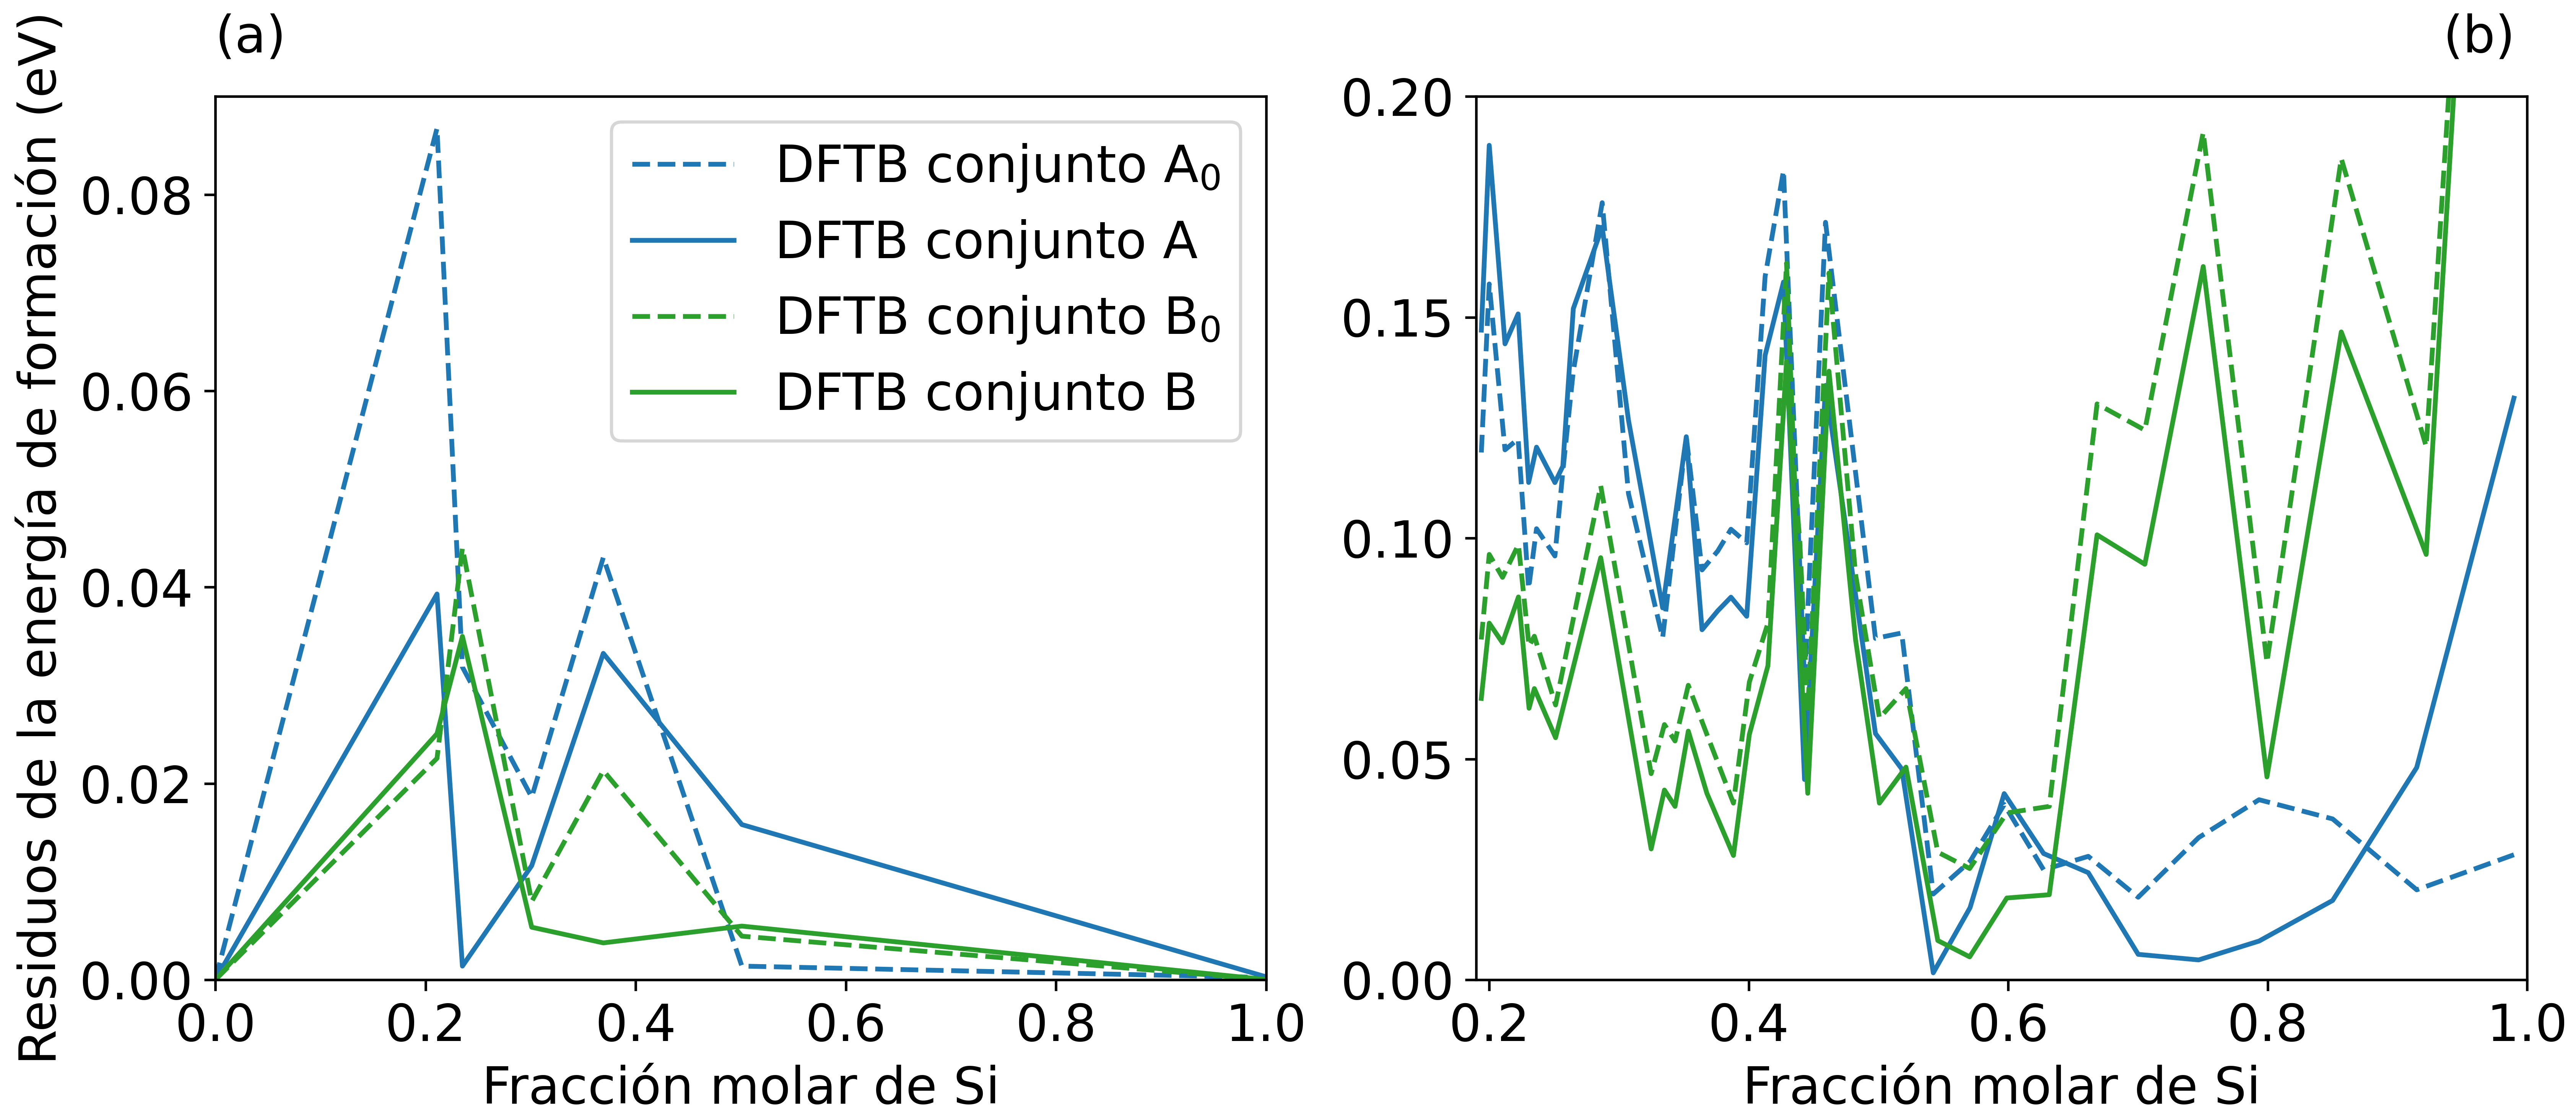
\includegraphics[width=\textwidth]{Silicio/modelo/resultados/residuos/residuos.png}
    \caption{Residuos de las energías de formación obtenidos con DFTB (respecto a
    DFT) con los conjuntos de parámetros antes de la optimización de los pesos 
    $\xi$ (A$_0$ y B$_0$) y después de la misma (A y B). (a) Estructuras
    cristalinas de Li--Si. (b) Estructuras amorfas de Li$_x$Si.}
    \label{fig:residuos}
\end{figure}
